In this chapter, the influence of different build parameter settings on the performance of the generation process and the resulting choreography models is examined. As measure for the performance of a choreography generation process that is constraint by parametric constraints as well as imposed compliance rules (see Chapter \ref{sec:constraints}), the number of necessary iterations for a successful generation is adducted. The iteration limitation is thereby set to ten. After ten iterations, the choreography generation is marked as failed. For the examination of the generation process that is only constraint by parametric constraints, the necessary duration for a successful build is used as measure, because the generation algorithm ensures that a model generation without imposed compliance rule will always result in a successful model within one iteration. In the following, first, the performance dependent on the parametric constraints is analyzed, and afterwards, the influence of different compliance rule settings, in conjunction with parametric constraints, is examined. In order to obtain representative results, each parameter configuration is run with 100 repetitions, if not stated otherwise.\\

Figure \ref{fig:anal_gateways} illustrates the influence of the number of parallel gateways onto the duration of a choreography model generation with 100 interactions. It shows that the generation duration is increasing linear to the number of gateway nodes included in the model. It also shows that there is no significant difference between the respective gateway types and also the combination between parallel and exclusive gateways (equal proportion). The generation duration increase is expected, because the more gateways are in the model, the more branches are created, and the more branches are in the model, the longer it takes to loop through the model to determine the number of free or reserved interactions.\\

\begin{figure}[htb]
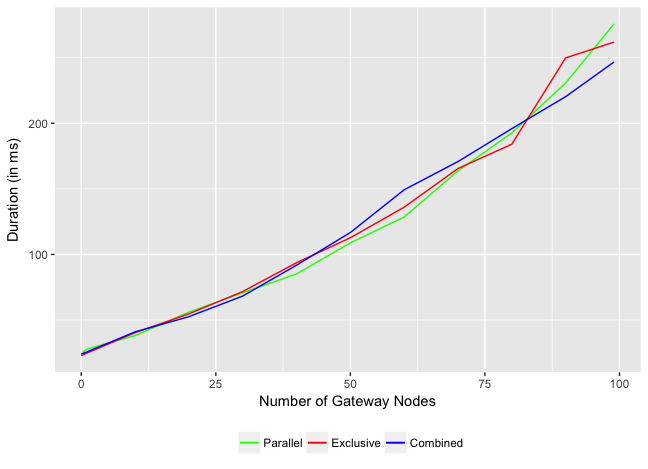
\includegraphics[width=1\textwidth]{src/images/analysis_gateways.png}
\caption{Choreography model generation duration depending on the number of gateway nodes}
\label{fig:anal_gateways}
\end{figure}

Figure \ref{fig:anal_branching} illustrates the influence of the max. branching parameter (see Section \ref{sec:param_constraints}) on the duration of a choreography model generation with 400 interactions and 20 gateway nodes. The graph shows that the generation duration is increasing linear to the increase of the max. branching parameter. The explanation for this is the same as for the influence of the number of gateway nodes. With the increase of the max. branching parameter, the number of branches in the build increases (premised that there are enough free interactions), and therefore the algorithms which loop through the branches consume more time.

\begin{figure}[htb]
\centering
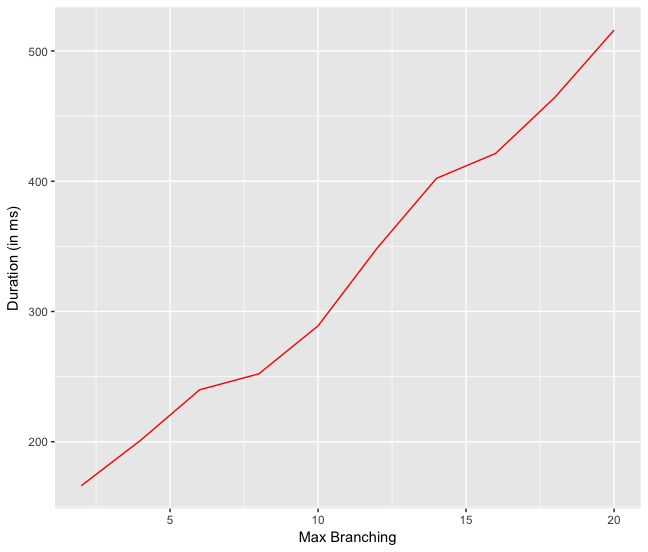
\includegraphics[width=0.9\textwidth]{src/images/analysis_branching.png}
\caption{Choreography model generation duration depending on the max. branching parameter}
\label{fig:anal_branching}
\end{figure}

For the analysis of the influence of different compliance rules settings on the model generation process, a random compliance rule generator is used. By specifying a number of interactions and a number of compliance rules, the generator generates supported compliance rules between those interactions randomly, which are then tried to be imposed on the generated models. Figure \ref{fig:anal_ands1} illustrates the influence of the number of compliance rules on a model generation process with 100 interactions, 10 parallel gateways and max. branching set to 2. It shows that the number of compliance rules has no impact on a model generation which only includes parallel gateways (various amounts of parallel gateway nodes were analyzed). Each model generation process was successful within the first iteration. This result is expected, because in a model without exclusive paths, all four supported compliance rule patterns (see Section \ref{sec:conception_compliance}), taken individually, can be assigned to any position in the model as long as they are one the same path (not parallel to another). 

\begin{figure}[htb]
\centering
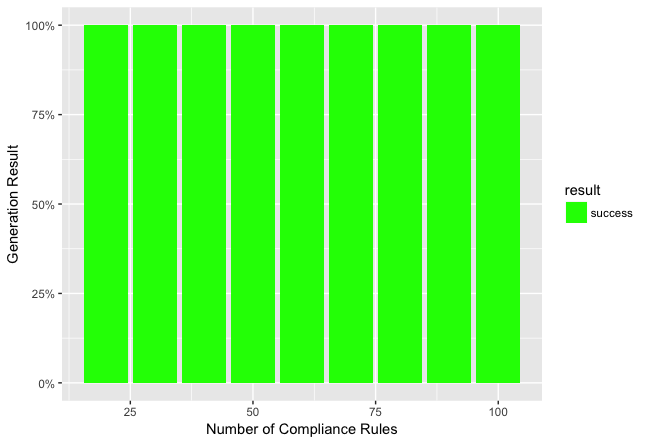
\includegraphics[width=0.9\textwidth]{src/images/ands_build_result.png}
\caption{Choreography model generation result depending on the number of compliance rules}
\label{fig:anal_ands1}
\end{figure}


This changes if a model generation includes exclusive gateways. Figure \ref{fig:anal_xors1} illustrates the influence of the number of compliance rules on a model generation process with 100 interactions, 10 exclusive gateways and max. branching set to 2. On the one hand, the result shows that the number of imposed compliance rule has no significant influence on the model generation success. On the other hand, on average only approx. 24\% of the generation processes are successful within 10 iterations. Figure \ref{fig:anal_xors2} shows the necessary iterations for the successful model generation processes depending on the number of specified compliance rules. This result is also expected, because the supported compliance rule patterns \textit{LeadsTo}, \textit{Precedes} and \textit{Universal} are hard to assign in a model with a lot of exclusive paths (see Definitions \ref{def:leadsto} - \ref{def:universal}). This is confirmed by examining the influence of the number of exclusive gateway onto a generation process restricted by 60 compliance rules, which is illustrated in Figure \ref{fig:anal_xors3}. The result shows that the more exclusive gateways, hence more exclusive paths, the more often the generation process fails within the specified iteration limitation. A successful generation is thereby also influenced by the level of dependency among the compliance rules. A high dependency among order patterns result in a more strict sequence order between the involved interactions, which makes it more difficult to assign them successfully.

\begin{figure}[htb]
\centering
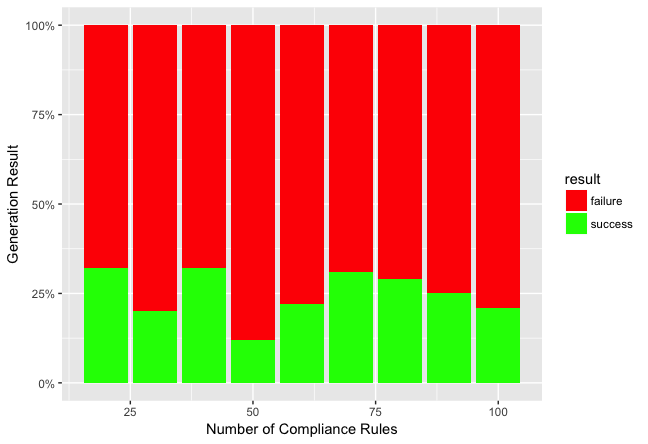
\includegraphics[width=0.9\textwidth]{src/images/xors_build_result.png}
\caption{Choreography model generation result depending on the number of compliance rules}
\label{fig:anal_xors1}
\end{figure}

\begin{figure}[H]
\centering
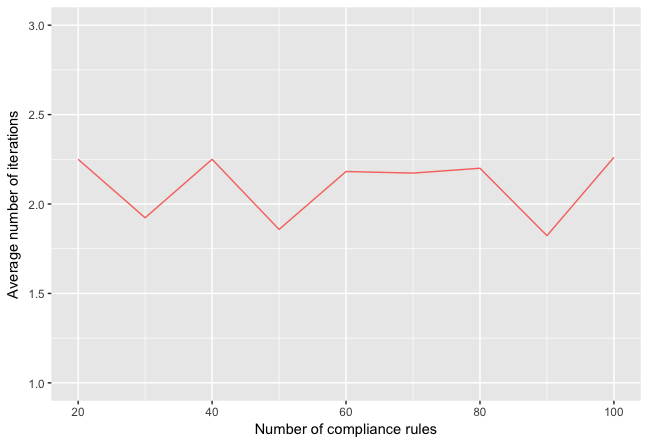
\includegraphics[width=0.9\textwidth]{src/images/xors_build_it.png}
\caption{Average iterations for successful generation}
\label{fig:anal_xors2}
\end{figure}

\begin{figure}[H]
\centering 
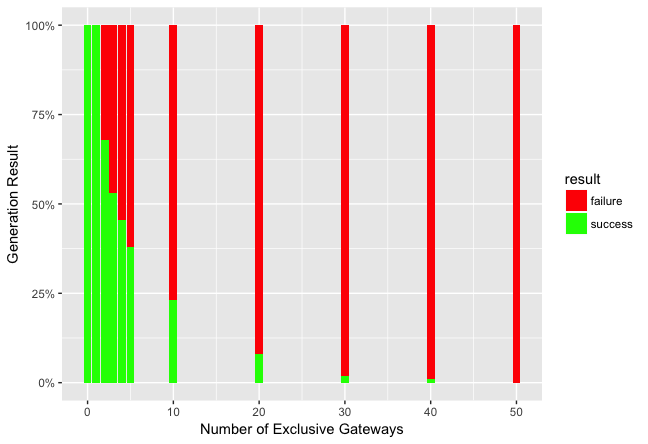
\includegraphics[width=0.9\textwidth]{src/images/xors_build_var.png}
\caption{Choreography generation result depending on the number of exclusive gateways and compliance rules}
\label{fig:anal_xors3}
\end{figure}

